%versi 3 (22-07-2020)
\chapter{Implementasi dan Pengujian}

Pada bab ini akan membahas tentang hasil dari rancangan antarmuka yang telah dibahas pada Bab \ref{chap:perancangan}. Pengimplementasian rancangan antarmuka agar dapat menampilkan perbandingan visual antara dua kelurahan di kota Bandung. Juga akan membahas tentang pengujian fungsional dan pengujian eksperimental.

\section{Implementasi}
\label{sec:implementasi}

Pada bagian ini akan membahas tentang perangkat keras dan perangkat lunak yang digunakan dalam membangaun perangkat lunak bedasarkan dari hasil rancangan antarmuka.

\subsection{Lingkungan Perangkat Keras}
Perangkat keras yang digunakan dalam mengimplementasi rancangan perangkat lunak memiliki spesifikasi sebagai berikut:
\begin{enumerate}
	\item Laptop : ASUS K55VD
	\item \textit{Processor} : Intel(R) Core(TM) i3-3110M CPU @2.40GHz(4CPUs), ~2.4GHz 
	\item RAM : 12GB 
	\item \textit{Solid State Drive} : 240 GB
\end{enumerate}


\subsection{Lingkungan Perangkat Lunak}

Perangkat lunak yang digunakan dalam mengimplementasi rancangan perangkat lunak memiliki spesifikasi sebagai berikut:
\begin{enumerate}
	\item \textit{Operating System} : Windows 10 Home Single Language
	\item \textit{Server} : web server Apache XAMPP version 3.3.0
	\item \textit{Client} : web browser Brave
	\item PHP \textit{Version} : 8.1.12
	\item DBMS : MySQL
	\item Visual Studio Code
	\item Laravel
\end{enumerate}

\subsection{Implementasi Basis Data}
\label{subsec:implmentasiBasisData}
Bagian ini terdapat implementasi basis data dalam perancangan perangkat lunak. Perangkat lunak akan memiliki data tabel berupa data\_wilayah yang digunakan untuk menyimpan data-data hasil eksperimen yang telah dilakukan kedalam database. Tabel data\_wilayah memiliki kode program seperti pada \ref{code:tabeldatawilayah}

\begin{lstlisting}[language=SQL, caption=Implementasi Tabel data\_wilayah,label={code:tabeldatawilayah}]
	CREATE TABLE `data_wilayah` (
	`id` int(11) NOT NULL,
	`nama_kelurahan` varchar(80) NOT NULL,
	`luas_kelurahan` float NOT NULL,
	`luas_kelurahan_prediksi` float NOT NULL,
	`luas_rth_kelurahan` float NOT NULL,
	`persentase_rth_kelurahan` float NOT NULL,
	`link_googlemaps` varchar(80) NOT NULL
	) ENGINE=InnoDB DEFAULT CHARSET=utf8mb4 COLLATE=utf8mb4_general_ci;
\end{lstlisting}

Lampiran \ref{lamp:basis-data} merupakan kode program yang digunakan dalam menampilkan seluruh implmentasi basis data pada perangkat lunak.

\section{Hasil Implementasi}
\label{sec:hasil-implementasi}
Implementasi perangkat lunak 'Pemvisualisasi Kelurahan Kota Bandung' dibangun dengan menggunakan bahasa pemrograman PHP dengan menggunakan \textit{framework} Laravel. Hasil  dari implementasi antarmuka saat perangkat lunak dijalankan pertama kali dapat di lihat pada gambar \ref{fig:home1}.
\begin{figure}[H]
	\centering
	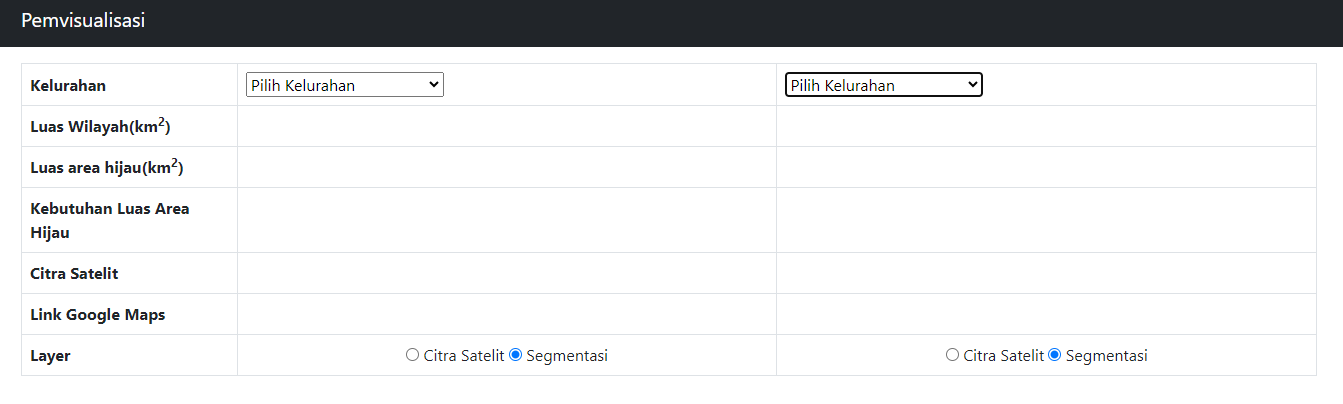
\includegraphics[width=0.8\textwidth]{Gambar/home1.png}
	\caption{Antarmuka Halaman Utama}
	\label{fig:home1}
\end{figure}

Pengguna  memilih kelurahan yang ingin dilihat dengan cara menekan \textit{dropdown} yang akan menampilkan pilihan-pilihan kelurahan di kota Bandung. Implementasi antarmuka saat memilih kelurahan dapat dilihat pada  gambar \ref{fig:home2}.
\begin{figure}[H]
	\centering
	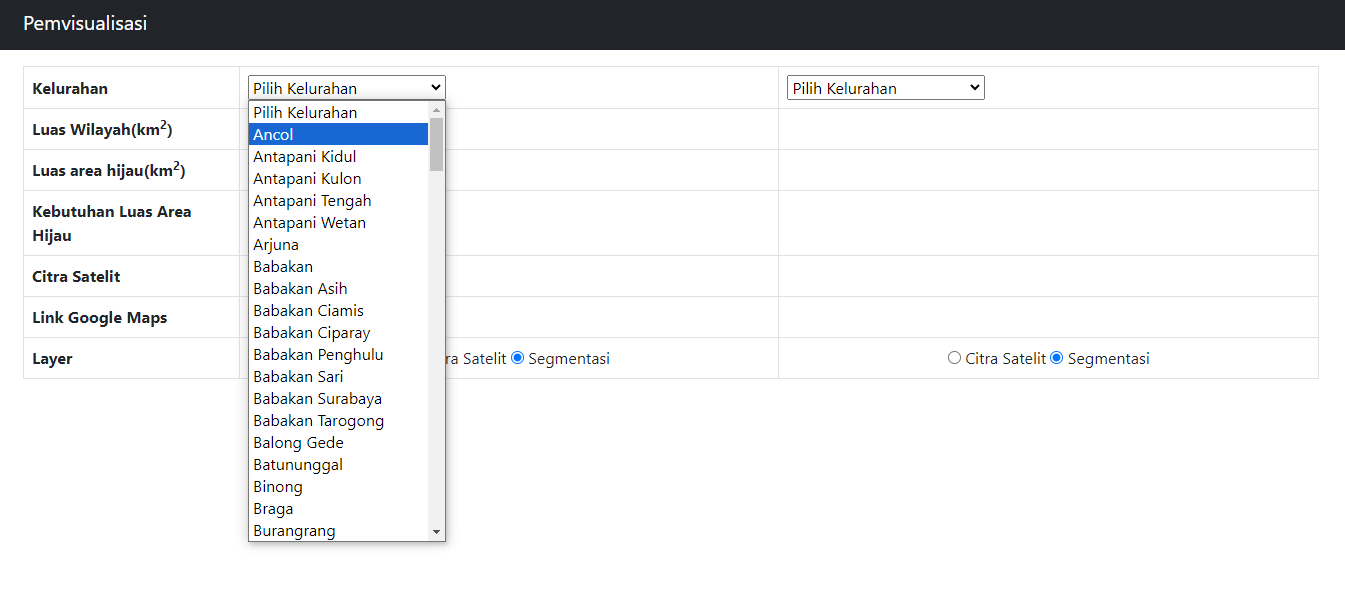
\includegraphics[width=0.8\textwidth]{Gambar/home2.png}
	\caption{Antarmuka Halaman Utama (\textit{Dropdown})}
	\label{fig:home2}
\end{figure} 
Setelah pengguna memilih kelurahan maka perangkat lunak akan menampilkan data dari setiap kelurahan dapat dilihat pada gambar \ref{fig:home3}.
\begin{figure}[H]
	\centering
	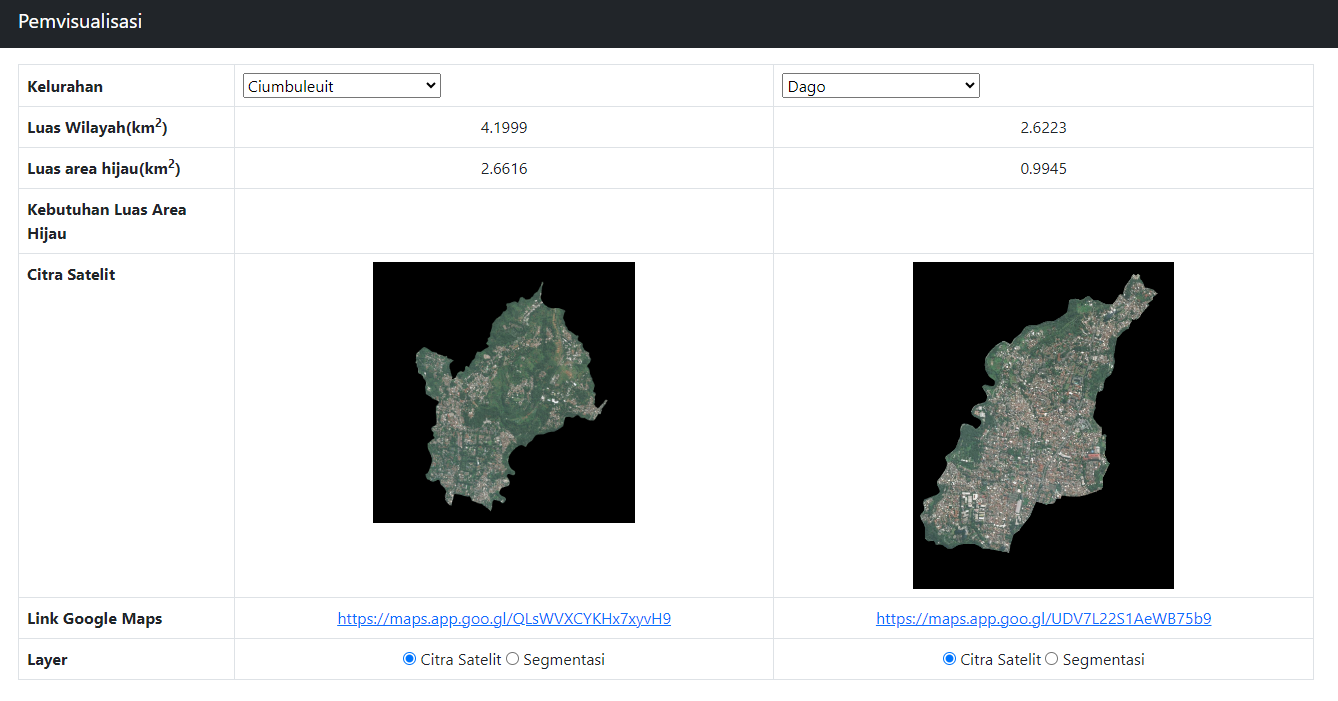
\includegraphics[width=0.8\textwidth]{Gambar/home3.png}
	\caption{Antarmuka Halaman Utama Menampilkan Data Kelurahan}
	\label{fig:home3}
\end{figure} 
Pengguna dapat memilih gambar hasil segmentasi area hijau dengan cara menekan \textit{radio-button} segmentasi,  maka tampilan rancangan antarmuka akan dapat dilihat seperti pada gambar \ref{fig:home5}
\begin{figure}[H]
	\centering
	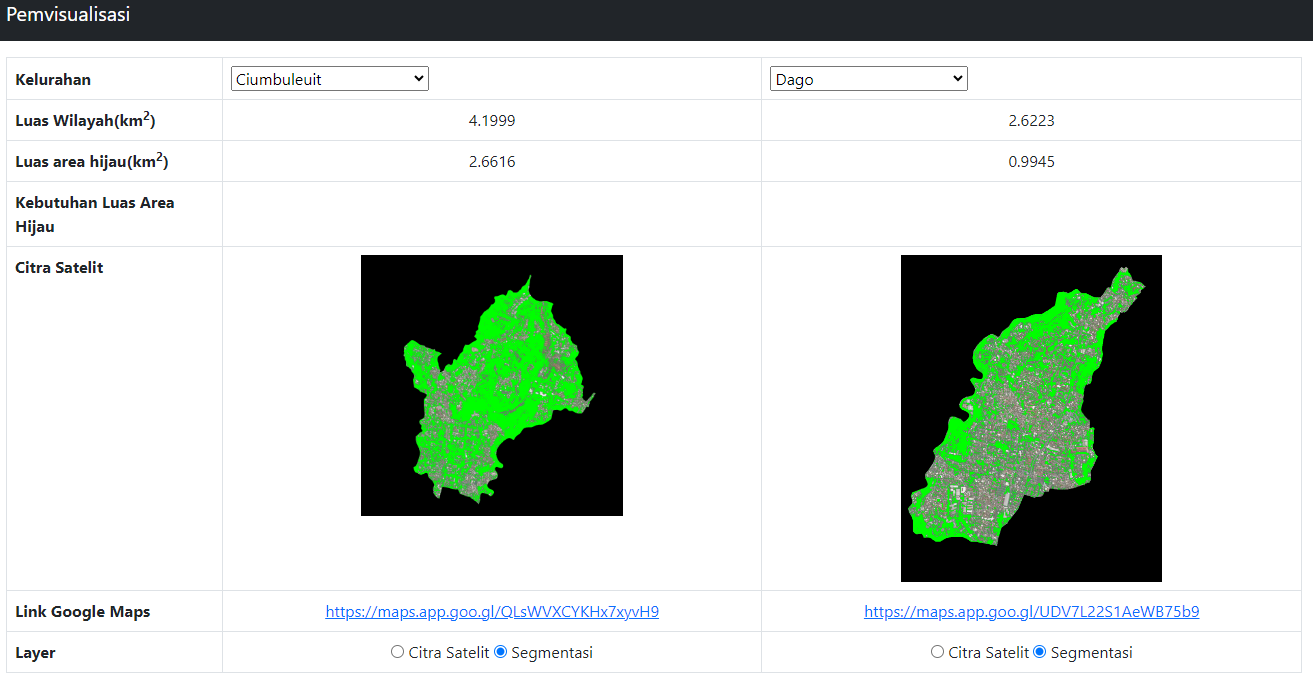
\includegraphics[width=0.8\textwidth]{Gambar/home5.png}
	\caption{Antarmuka Halaman Utama Menampilkan Gambar Citra Satelit Segementai}
	\label{fig:home5}
\end{figure} 

\section{Pengujian}
\label{sec:pengujian}
Pada bagian ini akan dibahas mengenai hasil pengujian perangkat lunak. Pengujian perangkat lunak merupakan satu set aktifitas yang direncanakan dan sistematis untuk menguji atau mengevaluasi kebenaran yang diinginkan\cite{rosa:11:pengujian}. Pengujian perangkat lunak memiliki tujuan untuk mengidentifikasi dan mengurangi potensi kesalahan, baik yang bersifat teknis maupun non-teknis. Selain itu, pengujian juga bertujuan untuk memastikan bahwa implementasi yang telah dilakukan berjalan dengan lancar, sehingga dapat diambil kesimpulan akhir mengenai kinerja perangkat lunak secara keseluruhan.

\subsection{Pengujian Fungsional}
Pengujian fugsional dilakukan untuk mengetahui apakah fungsi-fungsi, masukan dan keluaran dari pernagkat lunak sesuai dengan apa yang dibutuhkan. Hasil pengujian fungsional yang dilakukan terhadap dua buah kelurahan yaitu kelurahan Ciumbuleuit dapat dilihat pada tabel \ref{tab:pengujian-fungsional-ciumbuleuit} dan kelurahan Dago dapat dilihat pada tabel \ref{tab:pengujian-fungsional-dago}

\begin{comment}
	

\begin{table}[H]
	\centering
	\caption{Pengujian Fungsional}
	\label{tab:pengujian-fungsional}
	\resizebox{\textwidth}{!}{
		\begin{tabular}{|>{\hspace{0pt}}m{0.14\linewidth}|>{\hspace{0pt}}m{0.083\linewidth}|>{\hspace{0pt}}m{0.362\linewidth}|>{\hspace{0pt}}m{0.356\linewidth}|}
			\hline
			\textbf{Nama Fungsi}                         & \textbf{Kelurahan}  & \textbf{Hasil yang Diharapkan}                                                                                                            & \textbf{Hasil Pengujian}                                                                                                                  \\ 
			\hline
			Memilih kelurahan                            & Ciumbuleuit & Dropdown berisikan nama-nama kelurahan dan dapat dipilih                                                                                  & Dropdown berisikan nama-nama kelurahan dan dapat dipilih                                                                                  \\ 
			\hline
			Menampilkan Luas Wilayah                     & Ciumbuleuit  & Perangkat lunak akan menampilkan informasi berupa luas wilayah kelurahan yang dipilih                                                     & Perangkat lunak menampilkan informasi berupa luas wilayah kelurahan yang dipilih                                                          \\ 
			\hline
			Menampilkan Luas Area Hijau                  & Ciumbuleuit  & Perangkat lunak akan menampilkan informasi berupa luas area hijau kelurahan  yang dipilih                                                 & Perangkat lunak menampilkan informasi berupa luas area hijau kelurahan yang dipilih                                                       \\ 
			\hline
			Menampilkan Kebutuhan Luas Area Hijau        & Ciumbuleuit  & Perangkat lunak akan menampilkan informasi berupa kebutuhan luas area hijau kelurahan yang dipilih                                        & Perangat lunak belum bisa menampilkan informasi berupa kebutuhan luas area hijau kelurahan yang dipilih                                   \\ 
			\hline
			Menampilkan Gambar Citra Satelit             & Ciumbuleuit  & Perangkat lunak akan menampilkan gambar dari kelurahan                                                                                    & Perangkat lunak menampilkan gambar dari kelurahan yang dipilih                                                                            \\ 
			\hline
			Menampilkan Link Google Maps                 & Ciumbuleuit  & Perangkat lunak akan menampilkan link google maps dan jika ditekan akan alihkan kehalaman googlemaps sesuai dengan kelurahan yang dipilih & Perangkat lunak menampilkan link google maps dan jika ditekan akan dialihkan ke halaman google maps sesuai dengan kelurahan yang dipilih  \\ 
			\hline
			Menampilkan Gambar Segemetasi  Citra Satelit & Ciumbuleuit  & Perangkat lunak akan menampilkan gambar segmentasi citra satelit pada saat radio button segmentasi ditekan                                & Perangkan lunak menampilkan gambar segmentasi citra satelit pada saat radio button segementasi ditekan                                    \\
			\hline
		\end{tabular}}
\end{table}

\end{comment}

\begin{table}[H]
	\centering
	\caption{Pengujian Fungsional Kelurahan Ciumbuleuit}
	\label{tab:pengujian-fungsional-ciumbuleuit}
	\resizebox{\textwidth}{!}{
		\begin{tabular}{|>{\hspace{0pt}}m{0.14\linewidth}|>{\hspace{0pt}}m{0.083\linewidth}|>{\hspace{0pt}}m{0.362\linewidth}|>{\hspace{0pt}}m{0.356\linewidth}|}
			\hline
			\textbf{Nama Fungsi}                         & \textbf{Kelurahan}  & \textbf{Hasil yang Diharapkan}                                                                                                            & \textbf{Hasil Pengujian}                                                                                                                  \\ 
			\hline
			Memilih kelurahan                            & Ciumbuleuit & Dropdown berisikan nama-nama kelurahan dan dapat dipilih                                                                                  & Dropdown berisikan nama-nama kelurahan dan dapat dipilih                                                                                  \\ 
			\hline
			Menampilkan Luas Wilayah                     & Ciumbuleuit  & Perangkat lunak akan menampilkan informasi berupa luas wilayah kelurahan yang dipilih                                                     & Perangkat lunak menampilkan informasi berupa luas wilayah kelurahan yang dipilih                                                          \\ 
			\hline
			Menampilkan Luas Area Hijau                  & Ciumbuleuit  & Perangkat lunak akan menampilkan informasi berupa luas area hijau kelurahan  yang dipilih                                                 & Perangkat lunak menampilkan informasi berupa luas area hijau kelurahan yang dipilih                                                       \\ 
			\hline
			Menampilkan Kebutuhan Luas Area Hijau        & Ciumbuleuit  & Perangkat lunak akan menampilkan informasi berupa kebutuhan luas area hijau kelurahan yang dipilih                                        & Perangat lunak belum bisa menampilkan informasi berupa kebutuhan luas area hijau kelurahan yang dipilih                                   \\ 
			\hline
			Menampilkan Gambar Citra Satelit             & Ciumbuleuit  & Perangkat lunak akan menampilkan gambar dari kelurahan                                                                                    & Perangkat lunak menampilkan gambar dari kelurahan yang dipilih                                                                            \\ 
			\hline
			Menampilkan Link Google Maps                 & Ciumbuleuit  & Perangkat lunak akan menampilkan link google maps dan jika ditekan akan alihkan kehalaman googlemaps sesuai dengan kelurahan yang dipilih & Perangkat lunak menampilkan link google maps dan jika ditekan akan dialihkan ke halaman google maps sesuai dengan kelurahan yang dipilih  \\ 
			\hline
			Menampilkan Gambar Segemetasi  Citra Satelit & Ciumbuleuit  & Perangkat lunak akan menampilkan gambar segmentasi citra satelit pada saat radio button segmentasi ditekan                                & Perangkan lunak menampilkan gambar segmentasi citra satelit pada saat radio button segementasi ditekan                                    \\
			\hline
		\end{tabular}
	}
\end{table}

\begin{table}[H]
	\centering
	\caption{Pengujian Fungsional Kelurahan Dago}
	\label{tab:pengujian-fungsional-dago}
	\resizebox{\textwidth}{!}{
		\begin{tabular}{|>{\hspace{0pt}}m{0.14\linewidth}|>{\hspace{0pt}}m{0.083\linewidth}|>{\hspace{0pt}}m{0.362\linewidth}|>{\hspace{0pt}}m{0.356\linewidth}|}
			\hline
			\textbf{Nama Fungsi}                         & \textbf{Kelurahan}  & \textbf{Hasil yang Diharapkan}                                                                                                            & \textbf{Hasil Pengujian}                                                                                                                  \\ 
			\hline
			Memilih kelurahan                            & Dago & Dropdown berisikan nama-nama kelurahan dan dapat dipilih                                                                                  & Dropdown berisikan nama-nama kelurahan dan dapat dipilih                                                                                  \\ 
			\hline
			Menampilkan Luas Wilayah                     & Dago  & Perangkat lunak akan menampilkan informasi berupa luas wilayah kelurahan yang dipilih                                                     & Perangkat lunak menampilkan informasi berupa luas wilayah kelurahan yang dipilih                                                          \\ 
			\hline
			Menampilkan Luas Area Hijau                  & Dago  & Perangkat lunak akan menampilkan informasi berupa luas area hijau kelurahan  yang dipilih                                                 & Perangkat lunak menampilkan informasi berupa luas area hijau kelurahan yang dipilih                                                       \\ 
			\hline
			Menampilkan Kebutuhan Luas Area Hijau        & Dago  & Perangkat lunak akan menampilkan informasi berupa kebutuhan luas area hijau kelurahan yang dipilih                                        & Perangat lunak belum bisa menampilkan informasi berupa kebutuhan luas area hijau kelurahan yang dipilih                                   \\ 
			\hline
			Menampilkan Gambar Citra Satelit             & Dago  & Perangkat lunak akan menampilkan gambar dari kelurahan                                                                                    & Perangkat lunak menampilkan gambar dari kelurahan yang dipilih                                                                            \\ 
			\hline
			Menampilkan Link Google Maps                 & Dago  & Perangkat lunak akan menampilkan link google maps dan jika ditekan akan alihkan kehalaman googlemaps sesuai dengan kelurahan yang dipilih & Perangkat lunak menampilkan link google maps dan jika ditekan akan dialihkan ke halaman google maps sesuai dengan kelurahan yang dipilih  \\ 
			\hline
			Menampilkan Gambar Segemetasi  Citra Satelit & Dago  & Perangkat lunak akan menampilkan gambar segmentasi citra satelit pada saat radio button segmentasi ditekan                                & Perangkan lunak menampilkan gambar segmentasi citra satelit pada saat radio button segementasi ditekan                                    \\
			\hline
		\end{tabular}
	}
\end{table}


\subsection{Pengujian Eksperimental}
\label{subsec:pengujian-eksperimental}

Pada tahap ini penguji diberikan kesempatan untuk menggunakan semua fitur yang ada pada Perangkat Lunak Pemvisualisasi Hasil Penelitian Area Hijau Kelurahan. Penguji yang melakukan pengujian ini merupakan masyarakat yang tinggal di daerah Kota Bandung. Tujuan dilakukannya pengujian ini adalah untuk menguji kemudahan dalam menjalankan perangkat lunak. Setelah penguji menggunakan Perangkat Lunak Pemvisualisasi Hasil Penelitian Area Hijau Kelurahan Kota Bandung, penguji diminta untuk mengisi kuesioner untuk memberikan tanggapan dan saran terhadap pengembangan perangkat lunak ini. Pertanyaan pada kuesioner ini adalah sebagai berikut:
\begin{enumerate}
	\item Apakah perangkat lunak berjalan dengan baik (tidak ada crash atau error) dan dapat menampilkan informasi tentang area hijau di kelurahan dengan mudah?
	\item Apakah perangkat lunak menyediakan perbandingan area hijau antara kelurahan?
	\item Seberapa mudah Anda dapat membandingkan data area hijau di beberapa kelurahan?
	\item Apakah terdapat visualisasi data seperti gambar kelurahan yang membantu Anda memahami distribusi area hijau di kelurahan?
	\item Seberapa memuaskan Anda dengan presentasi informasi tentang area hijau di kelurahan?
	\item Seberapa mudah website atau perangkat lunak ini digunakan untuk mengeksplorasi informasi tentang area hijau di kelurahan?
	\item Apakah hasil yang dikeluarkan sesuai dengan harapan?
	\item Saran yang ingin disampaikan
\end{enumerate}

